\documentclass[11pt]{standalone}
\usepackage{amssymb}
\usepackage{amsmath}
\usepackage[no-math]{fontspec}
\usepackage{unicode-math}
\usepackage{libertinus}
\usepackage{pgf,xcolor}
\usepackage{tikz}
\usetikzlibrary{arrows.meta, backgrounds}
\usepackage{pgfplots}
\pgfplotsset{compat=newest}

\definecolor{my_darkgray}{HTML}{484949}
\definecolor{my_lightgray}{HTML}{F3F4F4}
\definecolor{my_darkblue}{HTML}{005A94}
\definecolor{my_lightblue}{HTML}{CCDEE9}
\definecolor{my_yellow}{HTML}{FFEC7F}
\definecolor{my_red}{HTML}{E60000}
\definecolor{my_orange}{HTML}{E87846}

\begin{document}

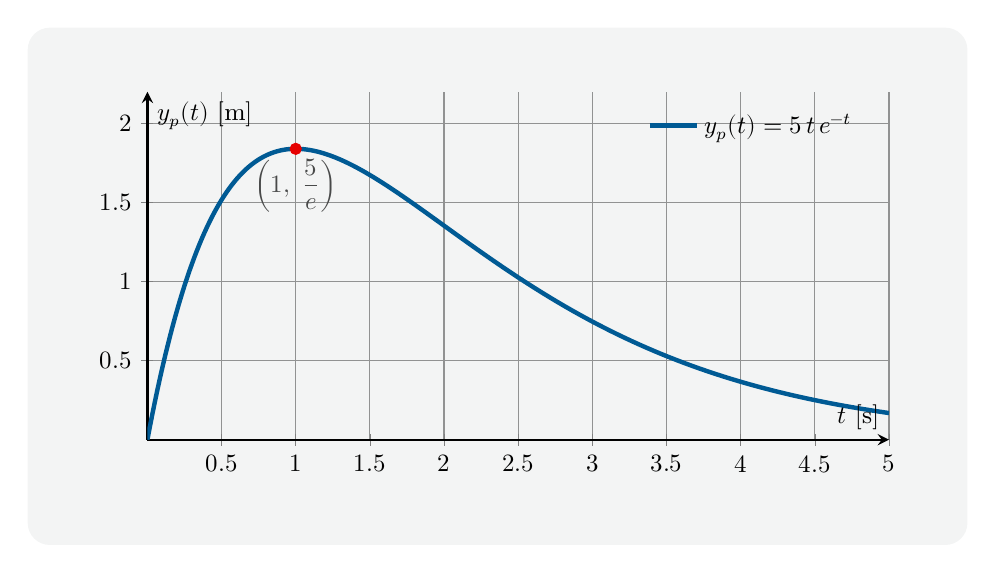
\begin{tikzpicture}[
    show background rectangle,
    background rectangle/.style={fill=my_lightgray, rounded corners=8pt},
    inner frame sep=0.8cm
]

\begin{axis}[
    width = 11cm,
    height = 6cm,
    axis lines = center,
    axis line style = {thick},
    xlabel = {$t~[\text{s}]$},
    ylabel = {$y_p(t)~[\text{m}]$},
    xlabel style = {font=\small},
    ylabel style = {font=\small},
    ticklabel style = {font=\small},
    grid = both,
    minor grid style = {draw=my_lightblue},
    major grid style = {draw=my_darkgray!60},
    xmin = 0,
    xmax = 5,
    ymin = 0,
    ymax = 2.2,
    legend style = {
        font=\small,
        at={(0.97,0.97)},
        anchor=north east,
        draw=none,
        fill=none,
        /tikz/every even column/.style={column sep=0.5em}
    },
    legend cell align = left,
    % axis equal hier bewusst weggelassen, damit der Anstieg und das
    % anschließende Abklingen von 5 t e^{-t} gut sichtbar sind.
]

% partikuläre Lösung im Resonanzfall: y_p(t) = 5 t e^{-t}
\addplot[
    draw = my_darkblue,
    ultra thick,
    samples = 300,
    domain = 0:5
]
{5*x*exp(-x)};
\addlegendentry{$y_p(t) = 5\,t\,e^{-t}$};

% Maximum bei t = 1, y = 5/e \approx 1.839
\addplot[
    only marks,
    mark = *,
    mark size = 2.0pt,
    draw = my_red,
    fill = my_red
]
coordinates {(1, 1.839)};
\node[my_darkgray, font=\small, anchor=north]
    at (axis cs:1, 1.839)
    {$\displaystyle\left(1,\;\frac{5}{e}\right)$};

\end{axis}

\end{tikzpicture}

\end{document}